\documentclass[pdf]{beamer}
\usepackage{graphicx}
\mode<presentation>{\usetheme{Warsaw}}
\title{A Study in the Calculus of Real Addition}
\subtitle{Leibniz's Algebra of Terms}
\author{Paul~Oppenheimer}
\subject{Linguistics}
\AtBeginSubsection
{
  \begin{frame}<beamer>{Outline}
    \tableofcontents[currentsection,currentsubsection]
  \end{frame}
}
\beamerdefaultoverlayspecification{<+->}
\begin{document}
\begin{frame}
  \titlepage
\end{frame}
\begin{frame}{Outline}
  \tableofcontents[pausesections]
\end{frame}
\section{Leibniz On the Calculus of Real Addition}
\subsection{The source}
\begin{frame}{The Source}{}
  \begin{itemize}
  \item G.W.~Leibniz (after 1690), ``A Study In the Calculus of Real Addition'',  {\em Leibniz: Logical Papers} (edited by G.H.R.~Parkinson), Oxford, 1966, 131--144.
  \end{itemize}
\end{frame}
\begin{frame}{Leibniz Portrait}
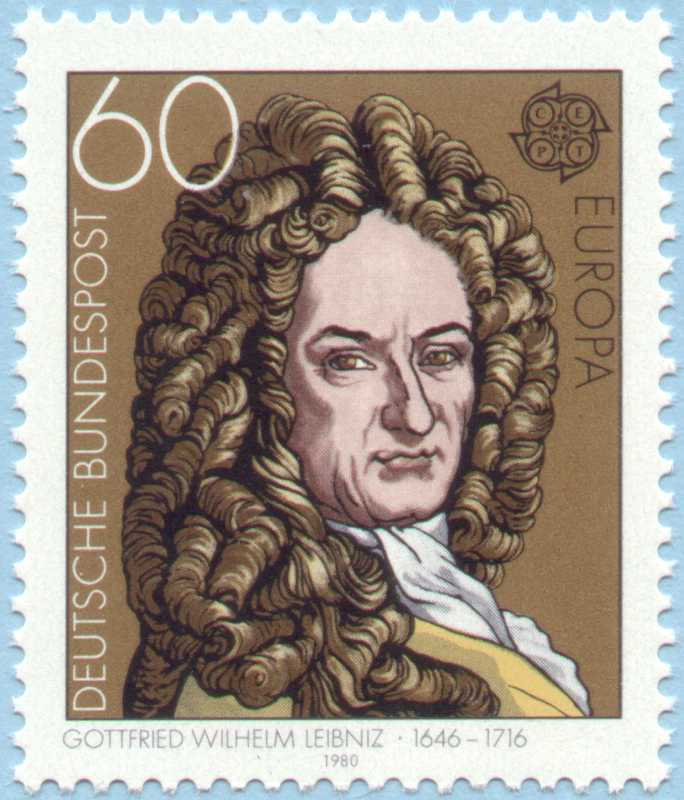
\includegraphics{leibniz2}
\end{frame}
\begin{frame}{A Calculus of Real Addition.}
\end{frame}
\end{document}
